\section{システムの動作確認}
\subsection{動作確認方法}

他の学生に協力してもらい，動作確認を行った．具体的には，椅子に座ってもらい光センサBを衣服に，脈拍センサを人差し指に装着した．Processing側で表\ref{tab5}に示す項目を表示し，条件ごとに必要な情報を記録した．動作確認をする条件は覚醒時，覚醒度低下時，起床時，誤使用時，暗所にいる時に分けて実施し，それぞれの確認事項，確認項目，確認方法を次の通りとした．
\begin{table}[tb]
\caption{Processingで表示する項目と詳細}
\label{tab5}
\centering
\begin{tabular}{l|l}\hline
表示する項目&詳細\\ \hline
Mod& 暗所モードなら1，それ以外なら0を表示する\\
State&\begin{tabular}{l}居眠り判定なら1，誤使用判定なら2，\\
それ以外なら0を表示する\end{tabular}\\
Data\_B\_var&5秒間ごとの光センサBの分散を数値で表示する\\
Data\_B&現在の光センサBの値を数値で表示する\\
Ambient\_Light&現在の環境光を数値で表示する\\
myBPM&現在のBPMを数値で表示する\\
LP& LPを表示する\\
RRIのグラフ&縦軸RRI，横軸時間のグラフを表示する\\
F-stressのグラフ&縦軸F-stress，横軸時間のグラフを表示する\\
光センサAのグラフ&縦軸光センサの値，横軸時間のグラフを表示する\\
光センサBのグラフ&縦軸光センサの値，横軸時間のグラフを表示する\\ \hline
\end{tabular}
\end{table}

\noindent{\gtbf{覚醒時}}\\
被験者が起きている時にセンサを取り付け記録する．
\begin{itemize}
\item \textmg{確認事項}
\begin{itemize}
\item RRIやF-stressがどのような値を取るのか
\item LPの各点が理論通りに散らばって表示されるのか
\item 光センサAとBはどのように変化するか
\item 具体的な環境光の値はいくつか
\end{itemize}
\item \textmg{確認項目}
\begin{itemize}
\item LP
\item RRI
\item F-stressのグラフ
\item 光センサのグラフ
\item Ambient\_Light
\item State
\end{itemize}
\end{itemize}

\noindent{\gtbf{覚醒度低下時}}\\
被験者がうとうとしている時の確認項目を記録する．
\begin{itemize}
\item \textmg{確認事項}
\begin{itemize}
\item RRIやF-stressがどのような値を取るのか
\item LPの各点が理論通りに右上に集まって表示されるのか
\item 光センサAとBはどのように変化するか
\item 具体的な環境光の値はいくつか
\end{itemize}
\item \textmg{確認項目}
\begin{itemize}
\item LP
\item RRI
\item F-stressのグラフ
\item 光センサのグラフ
\item Ambient\_Light
\end{itemize}
\end{itemize}

\noindent{\gtbf{起床時（居眠り判定）}}\\
被験者の覚醒度が低下していき，本装置によって居眠りが検知・防止された際の確認項目を記録する．
\begin{itemize}
\item \textmg{確認事項}
\begin{itemize}
\item 本装置で居眠りを判定し，モータを回すことで実際に被験者を起こすことができたか
\item 被験者が目覚めた後，モータは止まったか
\item RRIやF-stress，光センサのグラフには，起床前と起床後でどのような変化があるか
\item LPは覚醒度低下時に比べ，どのように変化したか
\item その時の具体的な環境光の値はいくつか
\item 居眠り判定としてStateが0から1に変化したか
\item 起床した際，Stateが1から0に戻ったか
\end{itemize}
\item \textmg{確認項目}
\begin{itemize}
\item LP
\item RRI
\item F-stressのグラフ
\item 光センサのグラフ
\item Ambient\_Light
\item モータの様子
\item 被験者の様子
\item State
\end{itemize}
\end{itemize}

\noindent{\gtbf{誤使用時}}\\
わざと姿勢を悪くしてもらい，その時の確認項目を記録する．
\begin{itemize}
\item \textmg{確認事項}
\begin{itemize}
\item 誤使用時（State = 2）を検知し，モータで警告できるか
\item 被験者が使用法や姿勢を直した際，Stateは0に戻り，モータの回転は止まったか
\end{itemize}
\item \textmg{確認項目}
\begin{itemize}
\item 光センサのグラフ
\item モータの様子
\item State
\item Data\_B\_var
\end{itemize}
\end{itemize}

\noindent{\gtbf{暗所にいる時}}\\
本装置を稼働したまま，部屋の照明を消す．
\begin{itemize}
\item \textgt{確認事項}
\begin{itemize}
\item 暗所を検知し，Modeを0から1へ切り替えられるか
\item 暗所の際，モータが回転しないか
\item 光センサA，Bともに値が低くなるか
\end{itemize}
\item \textgt{確認項目}
\begin{itemize}
\item Mode
\item 光センサのグラフ
\item モータの様子
\end{itemize}
\end{itemize}


\subsection{実行結果}
\subsubsection{覚醒時の動作}

覚醒時のLPを図\ref{fig10}，RRIを図\ref{fig11}，F-stressを図\ref{fig12}，光センサのグラフを図\ref{fig13}に示す．
この時のAmbient\_Lightの値は54であり，State は0であった．図\ref{fig10}に示すようにLPの各点は，200msから1000msの間にあり，ばらつきが見られた．図\ref{fig11}に示すRRIは6秒から15秒，39秒から50秒にかけて変動があり，図\ref{fig12}に示すF-stressも同様の時間に値の変動が見られた．図\ref{fig13}に示す光センサAの値は0秒から50秒にかけて54と変動はなかった．光センサBのグラフは，頭の動きに合わせ，非周期的な波形をしていることが読み取れる．

\begin{figure}[p]
\begin{center}
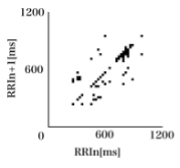
\includegraphics[width=5cm, clip]{fig10.png}
\caption{覚醒時のLP}
\label{fig10}
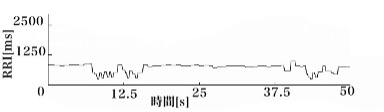
\includegraphics[width=8cm, clip]{fig11.png}
\caption{覚醒時のRRI}
\label{fig11}
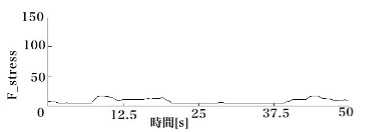
\includegraphics[width=8cm, clip]{fig12.png}
\caption{覚醒時のF-stress}
\label{fig12}
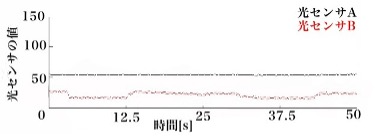
\includegraphics[width=8cm, clip]{fig13.png}
\caption{覚醒時の光センサ}
\label{fig13}
\end{center}
\end{figure}

\subsubsection{覚醒度低下時の動作}

覚醒度低下時のLPを図\ref{fig14}，RRIを図\ref{fig15}，F-stressを図\ref{fig16}，光センサのグラフを図\ref{fig17}に示す．この時のAmbient\_Lightの値は55であった．図\ref{fig14}に示すLPの各点は，$RRI_n-RRI_{n+1}$平面上において右上に集まってプロットされた．図\ref{fig15}に示すRRIの値は720msから900msの間を動き，図\ref{fig11}に示すほど変動していないことが読み取れる．図\ref{fig16}に示すF-stressは，0秒から50秒にかけて0に近い値を取っており，図\ref{fig12}に比べると変動が小さい．図\ref{fig17}に示す光センサAの値は，0秒から50秒にかけて55と変動しておらず，光センサBのグラフは，図\ref{fig13}と異なり，一定周期の波の形をとっていることが読み取れる．

\begin{figure}[p]
\begin{center}
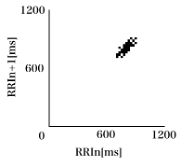
\includegraphics[width=5cm, clip]{fig14.png}
\caption{覚醒度低下時のLP}
\label{fig14}
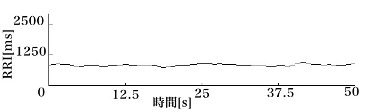
\includegraphics[width=8cm, clip]{fig15.png}
\caption{覚醒時低下時のRRI}
\label{fig15}
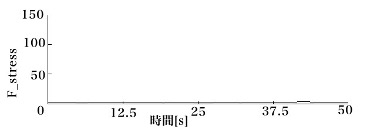
\includegraphics[width=8cm, clip]{fig16.png}
\caption{覚醒時低下時のF-stress}
\label{fig16}
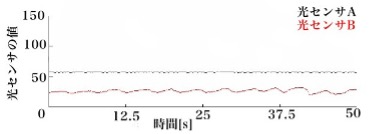
\includegraphics[width=8cm, clip]{fig17.png}
\caption{覚醒時低下時の光センサ}
\label{fig17}
\end{center}
\end{figure}

\subsubsection{起床時の動作}

本装置によって起床した時のLPを図\ref{fig18}，RRIを図\ref{fig19}，F-stressを図\ref{fig20}，光センサのグラフを図\ref{fig21}に示す．この時，Ambient\_Lightの値は49であった．Stateは28秒に0から1へ，31秒に1から0へと変化した．同時に28秒からモータが回転し，31秒にモータの回転が止まった．図\ref{fig18}に示すLPの各点の多くは，$RRI_n-RRI_{n+1}$平面上において右上に集中していることが読み取れるが，図\ref{fig14}に比べ，左下方向にばらつき始めていることがわかる．図\ref{fig19}に示すRRIにおいて，0秒から30.2秒にかけて値が緩やかに変化しているが，30.2秒から値の変動が大きくなっていることがわかる．同様に図\ref{fig20}に示すF-stressの値は，0秒から30.5秒にかけて0に近い値を取っていたが，30.5秒から変動を見せ，値が3から15へと大きくなっていることがわかる．図\ref{fig21}に示す光センサＡの値は0秒から50秒にかけて49と一定である．一方，光センサＢのグラフは0秒から25秒にかけて周期的な波形をしていた．しかし，25秒から27秒にかけて値が徐々に小さくなった．27秒から29.5秒にかけて0に近い値を取っていたが，29.5秒から37.5秒かけて値が0から20へと増加していることが読み取れる．また，被験者は0秒から25秒にかけてうとうとしていたが，25秒から30秒にかけて前かがみになり，30秒から31秒の間に目覚めた．

\begin{figure}[p]
\begin{center}
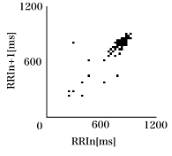
\includegraphics[width=5cm, clip]{fig18.png}
\caption{起床時のLP}
\label{fig18}
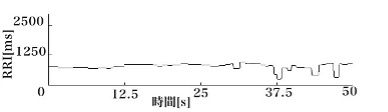
\includegraphics[width=8cm, clip]{fig19.png}
\caption{起床時のRRI}
\label{fig19}
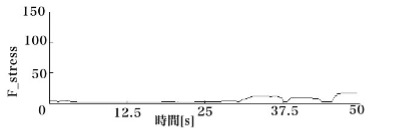
\includegraphics[width=8cm, clip]{fig20.png}
\caption{起床時のF-stress}
\label{fig20}
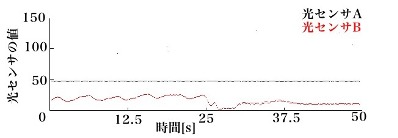
\includegraphics[width=8cm, clip]{fig21.png}
\caption{起床時の光センサ}
\label{fig21}
\end{center}
\end{figure}

\subsubsection{誤使用時の動作}

被験者は30秒から31秒にかけて光センサBの値が光センサAの値よりも大きくなるよう，姿勢を変えた．誤使用時の光センサのグラフを図\ref{fig22}に示す．図\ref{fig22}から光センサBの値が30秒から31秒にかけて光センサAの値よりも大きくなっていることがわかる．また，42秒から43秒にかけて光センサＢの値が，光センサＡの値よりも小さくなっていることがわかる．

0秒から30秒にかけてStateは0であったが，31秒からStateは2に変わった．Stateが2に変わると同時にモータが回転を始めた．被験者は42秒から43秒にかけて姿勢を戻した．44秒にStateは1から0へと戻った．Stateが0に戻ると同時に，モータの回転が止まった．

\begin{figure}[bt]
\begin{center}
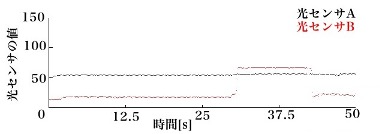
\includegraphics[width=8cm, clip]{fig22.png}
\caption{誤使用時の光センサ}
\label{fig22}
\end{center}
\end{figure}

\subsubsection{暗所にいる際の動作}

動作確認として21秒から23秒にかけて部屋の照明を消した．2つの光センサのグラフを図\ref{fig22}に示す．図\ref{fig22}から光センサAは50，光センサBは24の値を取っていたが，21秒から23秒にかけて共に値が小さくなっていることが読み取れる．また，25秒から4秒にかけて，両センサ共に0に近い値を取っていることがわかる． 0秒から24秒にかけてModeは0であったが，24秒から25秒にかけてModeは1に変化した．Modeが1の時，モータは回らなかった．
 
次に41秒から43秒にかけて部屋の証明を点灯した．図\ref{fig22}から41秒から43秒にかけて光センサAとBの値が共に増加していることがわかる．41秒から43秒の間にModeは1から0へ変化した．
\begin{figure}[bt]
\begin{center}
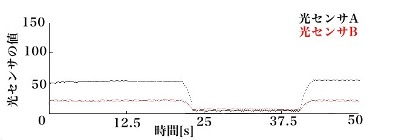
\includegraphics[width=8cm, clip]{fig23.png}
\caption{暗所にいる際の光センサ}
\label{fig23}
\end{center}
\end{figure}


